
\documentclass[journal,12pt,twocolumn]{IEEEtran}

\usepackage{setspace}
\usepackage{algpseudocode}
\usepackage{algorithm}
\usepackage{gensymb}
\singlespacing
\usepackage[cmex10]{amsmath}

\usepackage{amsthm}

\usepackage{mathrsfs}
\usepackage{txfonts}
\usepackage{stfloats}
\usepackage{bm}
\usepackage{cite}
\usepackage{cases}
\usepackage{subfig}
\usepackage{tikz}
\usepackage{longtable}
\usepackage{multirow}

\usepackage{enumitem}
\usepackage{mathtools}
\usepackage{steinmetz}
\usepackage{tikz}
\usepackage{circuitikz}
\usepackage{verbatim}
\usepackage{tfrupee}
\usepackage[breaklinks=true]{hyperref}
\usepackage{graphicx}
\usepackage{tkz-euclide}

\usetikzlibrary{calc,math}
\usepackage{listings}
    \usepackage{color}                                            %%
    \usepackage{array}                                            %%
    \usepackage{longtable}                                        %%
    \usepackage{calc}                                             %%
    \usepackage{multirow}                                         %%
    \usepackage{hhline}                                           %%
    \usepackage{ifthen}                                           %%
    \usepackage{lscape}     
\usepackage{multicol}
\usepackage{chngcntr}

\DeclareMathOperator*{\Res}{Res}

\renewcommand\thesection{\arabic{section}}
\renewcommand\thesubsection{\thesection.\arabic{subsection}}
\renewcommand\thesubsubsection{\thesubsection.\arabic{subsubsection}}

\renewcommand\thesectiondis{\arabic{section}}
\renewcommand\thesubsectiondis{\thesectiondis.\arabic{subsection}}
\renewcommand\thesubsubsectiondis{\thesubsectiondis.\arabic{subsubsection}}


\hyphenation{op-tical net-works semi-conduc-tor}
\def\inputGnumericTable{}                                 %%

\lstset{
%language=C,
frame=single, 
breaklines=true,
columns=fullflexible
}
\begin{document}


\newtheorem{theorem}{Theorem}[section]
\newtheorem{problem}{Problem}
\newtheorem{proposition}{Proposition}[section]
\newtheorem{lemma}{Lemma}[section]
\newtheorem{corollary}[theorem]{Corollary}
\newtheorem{example}{Example}[section]
\newtheorem{definition}[problem]{Definition}

\newcommand{\BEQA}{\begin{eqnarray}}
\newcommand{\EEQA}{\end{eqnarray}}
\newcommand{\define}{\stackrel{\triangle}{=}}
\bibliographystyle{IEEEtran}
\raggedbottom
\setlength{\parindent}{0pt}
\providecommand{\mbf}{\mathbf}
\providecommand{\pr}[1]{\ensuremath{\Pr\left(#1\right)}}
\providecommand{\qfunc}[1]{\ensuremath{Q\left(#1\right)}}
\providecommand{\sbrak}[1]{\ensuremath{{}\left[#1\right]}}
\providecommand{\lsbrak}[1]{\ensuremath{{}\left[#1\right.}}
\providecommand{\rsbrak}[1]{\ensuremath{{}\left.#1\right]}}
\providecommand{\brak}[1]{\ensuremath{\left(#1\right)}}
\providecommand{\lbrak}[1]{\ensuremath{\left(#1\right.}}
\providecommand{\rbrak}[1]{\ensuremath{\left.#1\right)}}
\providecommand{\cbrak}[1]{\ensuremath{\left\{#1\right\}}}
\providecommand{\lcbrak}[1]{\ensuremath{\left\{#1\right.}}
\providecommand{\rcbrak}[1]{\ensuremath{\left.#1\right\}}}
\theoremstyle{remark}
\newtheorem{rem}{Remark}
\newcommand{\sgn}{\mathop{\mathrm{sgn}}}
% \providecommand{\abs}[1]{\left\vert#1\right\vert}
% \providecommand{\res}[1]{\Res\displaylimits_{#1}} 
% \providecommand{\norm}[1]{\left\lVert#1\right\rVert}
% %\providecommand{\norm}[1]{\lVert#1\rVert}
% \providecommand{\mtx}[1]{\mathbf{#1}}
% \providecommand{\mean}[1]{E\left[ #1 \right]}
\providecommand{\fourier}{\overset{\mathcal{F}}{ \rightleftharpoons}}
%\providecommand{\hilbert}{\overset{\mathcal{H}}{ \rightleftharpoons}}
\providecommand{\system}{\overset{\mathcal{H}}{ \longleftrightarrow}}
	%\newcommand{\solution}[2]{\textbf{Solution:}{#1}}
\newcommand{\solution}{\noindent \textbf{Solution: }}
\newcommand{\cosec}{\,\text{cosec}\,}
\providecommand{\dec}[2]{\ensuremath{\overset{#1}{\underset{#2}{\gtrless}}}}
\newcommand{\myvec}[1]{\ensuremath{\begin{pmatrix}#1\end{pmatrix}}}
\newcommand{\mydet}[1]{\ensuremath{\begin{vmatrix}#1\end{vmatrix}}}
\numberwithin{equation}{subsection}
\def\putbox#1#2#3{\makebox[0in][l]{\makebox[#1][l]{}\raisebox{\baselineskip}[0in][0in]{\raisebox{#2}[0in][0in]{#3}}}}
     \def\rightbox#1{\makebox[0in][r]{#1}}
     \def\centbox#1{\makebox[0in]{#1}}
     \def\topbox#1{\raisebox{-\baselineskip}[0in][0in]{#1}}
     \def\midbox#1{\raisebox{-0.5\baselineskip}[0in][0in]{#1}}
\vspace{3cm}
\title{Assignment 1}
\author{Harsh Kabra - EE18BTECH11019}
\maketitle
% \newpage
\bigskip
Github repository
%
\begin{lstlisting}
https://github.com/harsh006/C-DS/tree/main
\end{lstlisting}
\setcounter{figure}{0}
\section{Problem}
In a directed acyclic graph with source vertex s, the quality-score of a directed path is defined to be the product of the weights of the edges on the path. Further, for a vertex v other than s, the quality-score of v is defined to be the maximum among the quality-scores of all the paths from s to v. The quality-score of s is assumed to be 1.\\

\begin{figure}[!h]
    \centering
    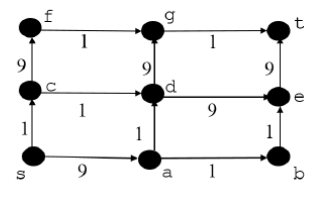
\includegraphics[scale=1]{figures/ee18btech11019_graph.PNG}
    \label{fig:verification}
\end{figure}
Then the sum of quality-scores of all vertices in the graph shown above is?
\section{Solution}
\subsection{\textbf{About the problem}}
\begin{itemize}

\item So, we are given a Directed Acyclic Graph (DAG), as shown in the above figure so we are supposed to find maximum of quality-scores for each node from a given source S.
\item Where each quality-score is found by multiplying weight of edge from one node to other node.
\item As the above problem, we have a single source and have to find Longest Path
\item Synonymous to longest path, here instead of addition of weights,we have multiplication and all positive values
\item We, will hence use \textbf{Bellman-Ford algorithm} to solve this problem.

\end{itemize}
\subsection{\textbf{About Bellman-Ford algorithm}}
\begin{itemize}

 \item The algorithm calculates longest paths in a bottom-up manner.That is,
 \item It first calculates the shortest distances which have at-most one edge from source to our current node in the path.
 \item Then, it calculates the shortest paths with at-most 2 edges, and so on. \item After the i-th iteration, the shortest paths with at most i edges in path are calculated. As,evident this to similar to BFS style of traversal.
 \item There can be maximum V–1 edges in any simple path, that is why the outer loop runs v – 1 times. Where, V = number of nodes.
\end{itemize}
\textbf{The exact steps are - }
\begin{itemize}
\item Initialize distances from the source to all vertices as negative infinity(lowest possible value) and distance to the source itself as
\begin{algorithm}
\begin{algorithmic}
\State $source \gets 0$
\State $cost \gets $[-INF]*N
\State $cost[source] \gets 1$
\end{algorithmic}
\end{algorithm}
\item This step calculates longest distances.\\

\begin{algorithm}
\begin{algorithmic}
    \State $it \gets 1$
    \While{$it \neq V-1$}
    \For{\State $e in $Adj[it]}
    \State $u \gets dest node$
    \State $w \gets weight$
    \If{$cost[v]*w$ > $cost[u]$}
    \State $cost[u]$ = $cost[v]*w$
    \EndIf
    \EndFor
    \State $it \gets it+1$
    \EndWhile
\end{algorithmic}
\end{algorithm}
\begin{itemize}


\item Looping through V-1 time \\
\item Inside the above loop, again Looping through each edge at each iteration and checking if the cost is higher any time.

\end{itemize}

\item Analyzing time complexity:\\
\begin{equation}
        T(n)  = O(n*(n-1)) \label{eq:runtime_eff}
        \implies O(n^{2})
\end{equation}

\end{itemize}
\subsection{\textbf{Solution}}
The following are the values we get after applying the above algorithm:\\
\begin{itemize}
\item dist (s, s) = 1\\
\item dist (s, a) = 9\\
\item dist (s, b) = 9\\
\item dist (s, c) = 1\\
\item dist (s, d) = 9\\
\item dist (s, e) = 81\\
\item dist (s, f) = 9\\
\item dist (s, g) = 81\\
\item dist (s, h) = 729\\
\end{itemize}
Therefore, finally sum of all the values = \textbf{929}\\
\textbf{Code can be found in:}
\begin{lstlisting}
https://github.com/harsh006/C-DS/tree/main/code
\end{lstlisting}
\end{document}